%==================== chapter3_24.tex ====================

\clearpage
\thispagestyle{plain}

\begingroup
\fontsize{16pt}{19.2pt}\selectfont
\justifying
\XeTeXlinebreakskip=0pt plus 1pt minus 0.5pt
\setlength{\parindent}{1.5cm}
\setlength{\parskip}{0pt}

% ---------- หัวข้อใหญ่ (ชิดซ้าย, หนา 16pt) ----------
\section*{Sequence Diagra}
\addcontentsline{toc}{section}{Sequence Diagra}

% ---------- เนื้อหา (จัดกระจายแบบไทย, ย่อหน้าแรก 1.5 ซม.) ----------
\indent Sequence Diagram เป็นแผนผังแสดงการทำงานแบบลำดับปฏิสัมพันธ์ โดยระบบประเมินปลากัดก่อนการแข่งขันโดยผู้เชี่ยวชาญ มีองค์ประกอบ Sequence Diagram ดังนี้

% ===== enumerate แบบ robust (ไม่ใช้ \dimexpr เพื่อกัน error) =====
\setlist[enumerate,1]{%
	label=\arabic*., align=left,
	leftmargin=1.5cm, labelindent=0pt,
	labelwidth=\LoneLabelWidth, labelsep=\LoneLabelSep,
	itemsep=0pt, topsep=0.5\baselineskip
}

% ระดับ 2: ให้คอลัมน์ข้อความตรงตามที่ตั้ง (ชิฟต์ด้วย \ExtraAlign)
\setlist[enumerate,2]{%
	label*=\arabic*., align=left,
	leftmargin=*,
	labelwidth=\LtwoLabelWidth, labelsep=\LtwoLabelSep,
	labelindent=\dimexpr \LoneContentCol + \ExtraAlign - \LtwoLabelWidth - \LtwoLabelSep\relax,
	itemsep=0pt, topsep=0pt
}
\setlist[enumerate,3]{%
	label*=\arabic*., align=left,
	leftmargin=*, labelsep=-0.6em,
	labelindent=-1em, % ให้คอลัมน์ข้อความตรงเส้นเดียวกับระดับ 2
	widest=9.9.9,
	itemsep=0pt, topsep=0pt
}

\begin{enumerate}
	\item การเข้าสู่ระบบ (User Sign In)
	\item ผู้ใช้ส่งปลากัด (พร้อม AI Analysis)
	\item Manager อนุมัติผู้สมัคร
	\item Expert ส่งผลประเมิน
\end{enumerate}

\vspace{\baselineskip}

\begin{figure}[h]
	\centering
	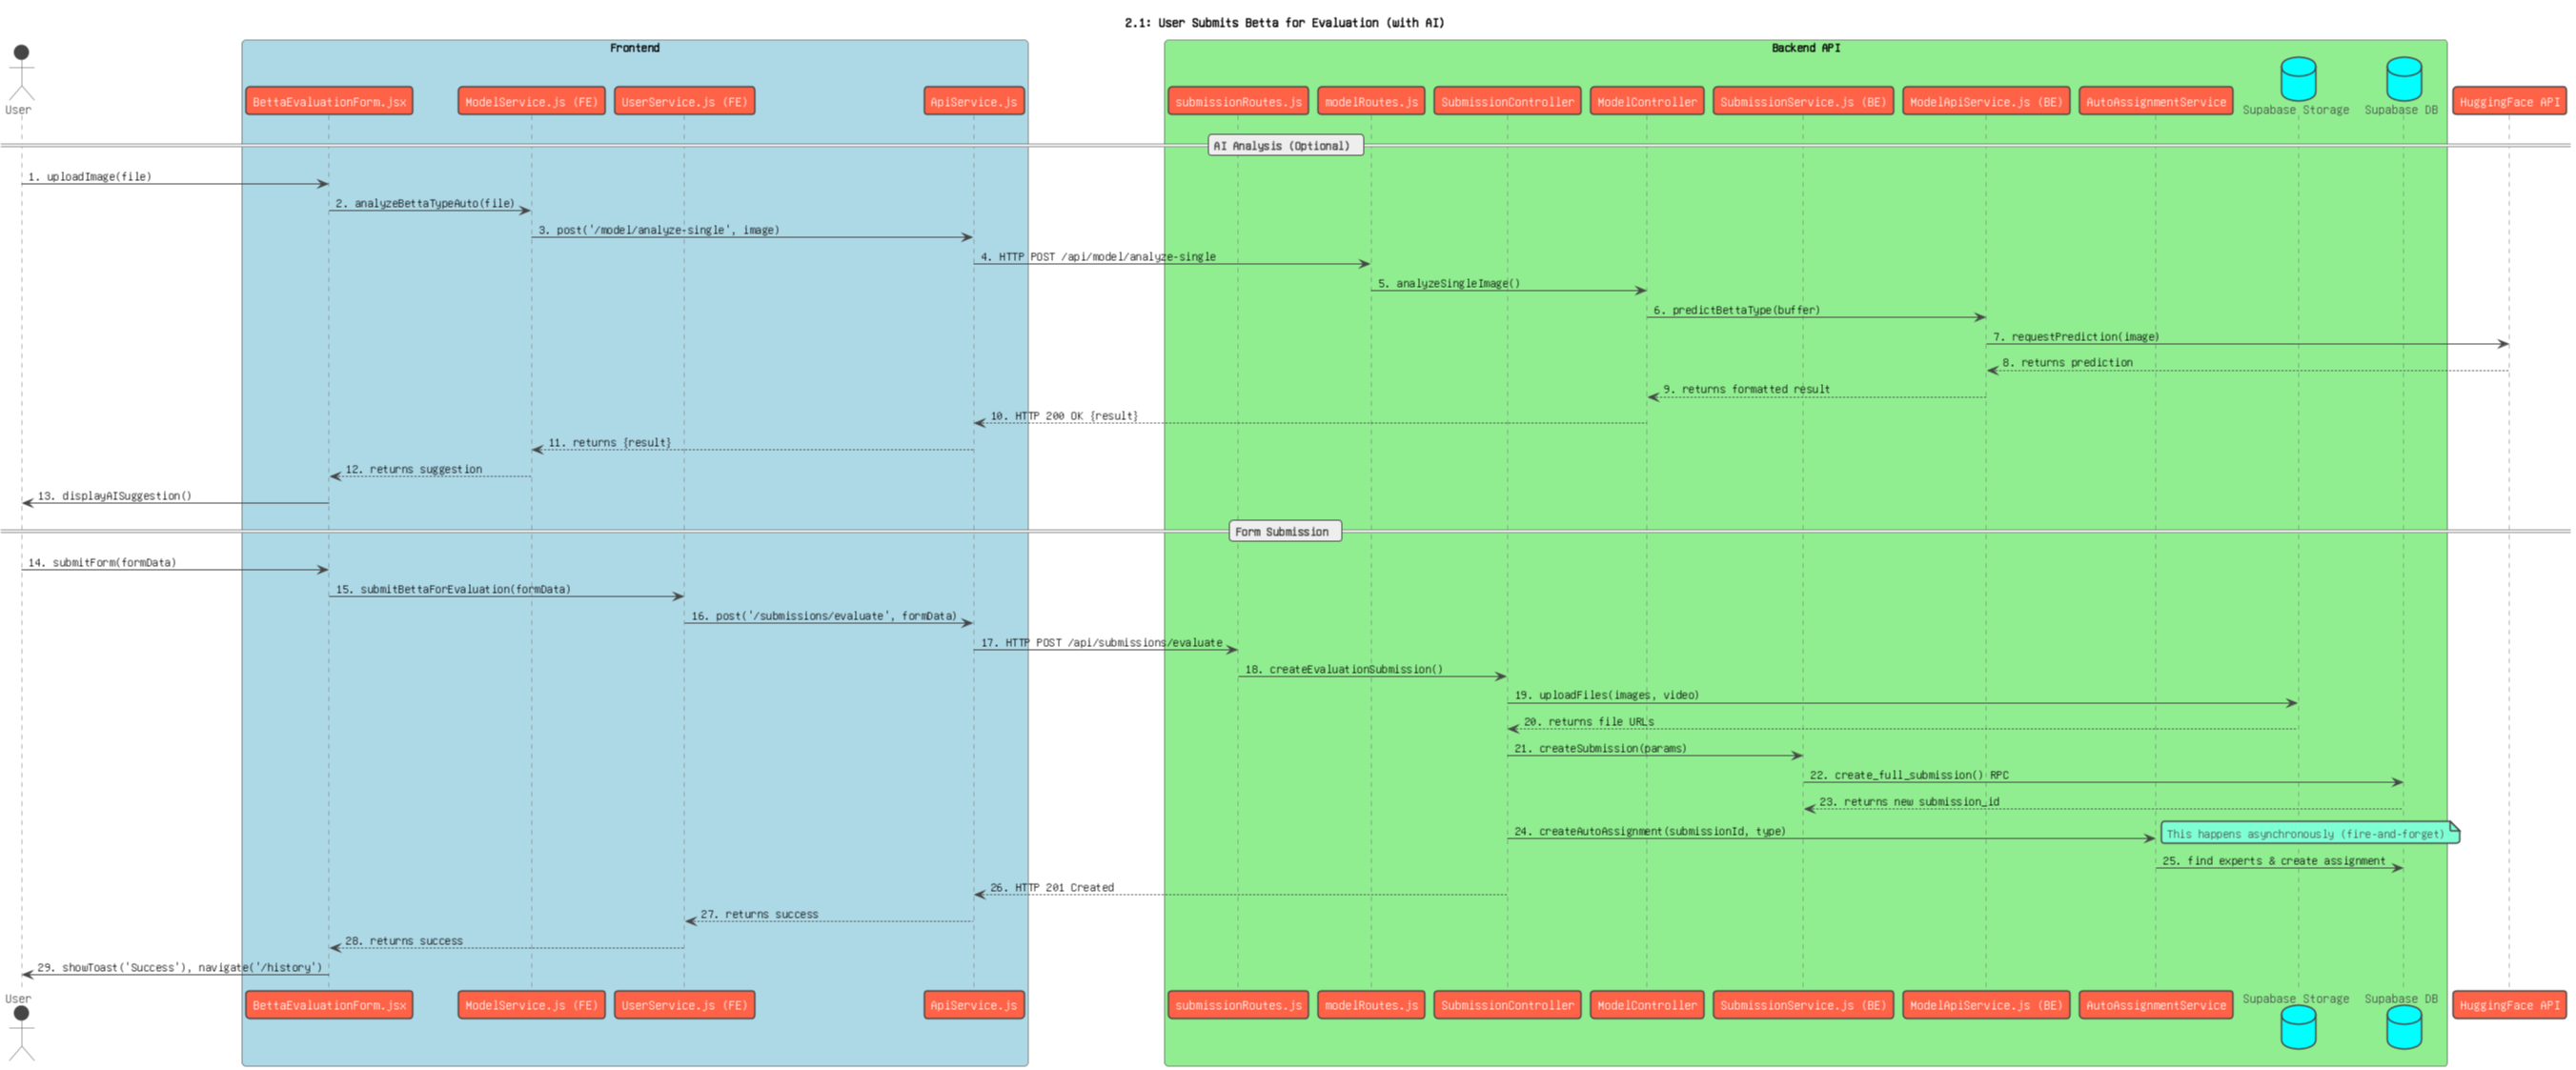
\includegraphics[width=0.8\linewidth]{S1.drawio}
	\caption{การเข้าสู่ระบบ (User Sign In)}
\end{figure}

\indent ไดอะแกรมนี้แสดงลำดับเหตุการณ์เมื่อผู้ใช้พยายามเข้าสู่ระบบ ตั้งแต่การกรอกข้อมูลไปจนถึงการตรวจสอบสิทธิ์และอัปเดตหน้าเว็บ

% --- ขั้นตอนการเข้าสู่ระบบ ---

\begin{sloppypar}
	\begin{enumerate}
		\item \textbf{ขั้นตอนการเข้าสู่ระบบ (User Sign In)}
		\begin{enumerate}
			\item User -> Login.jsx: ผู้ใช้กรอกอีเมลและรหัสผ่านในหน้า Login แล้วกดปุ่ม “เข้าสู่ระบบ”
			\item Login.jsx -> AuthContext: Component Login เรียกใช้ฟังก์ชัน signin() จาก AuthContext ซึ่งเป็นศูนย์กลางจัดการสถานะการล็อกอิน
			\item AuthContext -> authService.js (FE): AuthContext ส่งต่อคำสั่งไปยัง authService (ฝั่ง Frontend) เพื่อเริ่มกระบวนการล็อกอิน
			\item authService.js (FE) -> ApiService.js: authService เรียกใช้ ApiService ซึ่งเป็น Service กลางสำหรับส่ง HTTP Request ทั้งหมด โดยส่ง POST ไปยัง endpoint /auth/signin
			\item ApiService.js -> authRoutes.js (BE): ApiService ส่ง HTTP POST ไปยัง Backend API ที่ /api/auth/signin
			\item authRoutes.js (BE) -> AuthController: Router ฝั่ง Backend ส่งต่อคำขอไปยังฟังก์ชัน handleSignIn() ใน AuthController
			\item AuthController -> AuthService.js (BE): Controller เรียกใช้ AuthService ซึ่งดูแล Business Logic ของการเข้าสู่ระบบ
			\item AuthService.js (BE) -> Supabase: ส่งอีเมลและรหัสผ่านไปตรวจสอบกับ Supabase Auth
			\item Supabase -> AuthService.js (BE): ถ้าถูกต้อง ส่งข้อมูล user และ session (มี JWT Token) กลับมา
			\item AuthService.js (BE) -> Supabase: นำ user.id ไปค้นหาข้อมูลโปรไฟล์จากตาราง profiles
			\item Supabase -> AuthService.js (BE): ส่งข้อมูลโปรไฟล์ (เช่น role, ชื่อ, นามสกุล) กลับมา
			\item AuthService.js (BE) -> AuthController: ส่งผลลัพธ์สุดท้าย (token + profile) กลับให้ Controller
			\item AuthController -> ApiService.js: ส่ง HTTP 200 OK พร้อม token และ profile กลับไปยัง Frontend
			\item ApiService.js -> authService.js (FE): ApiService ส่งต่อผลลัพธ์ให้ authService
			\item authService.js (FE) -> authService.js (FE): บันทึก Token และโปรไฟล์ลงใน localStorage ของเบราว์เซอร์
			\item authService.js (FE) -> AuthContext: ส่งข้อมูล profile กลับให้ AuthContext
			\item AuthContext -> AuthContext: อัปเดต state ภายใน โดยตั้งค่า user และ isAuthenticated = true
			\item AuthContext -> Login.jsx: แจ้งผลสำเร็จกลับไปยัง Component Login
			\item Login.jsx -> User: นำทางผู้ใช้ไปยัง Dashboard ที่เหมาะสมกับ Role
		\end{enumerate}
	\end{enumerate}
\end{sloppypar}

\newpage

\begin{figure}[h]
	\centering
	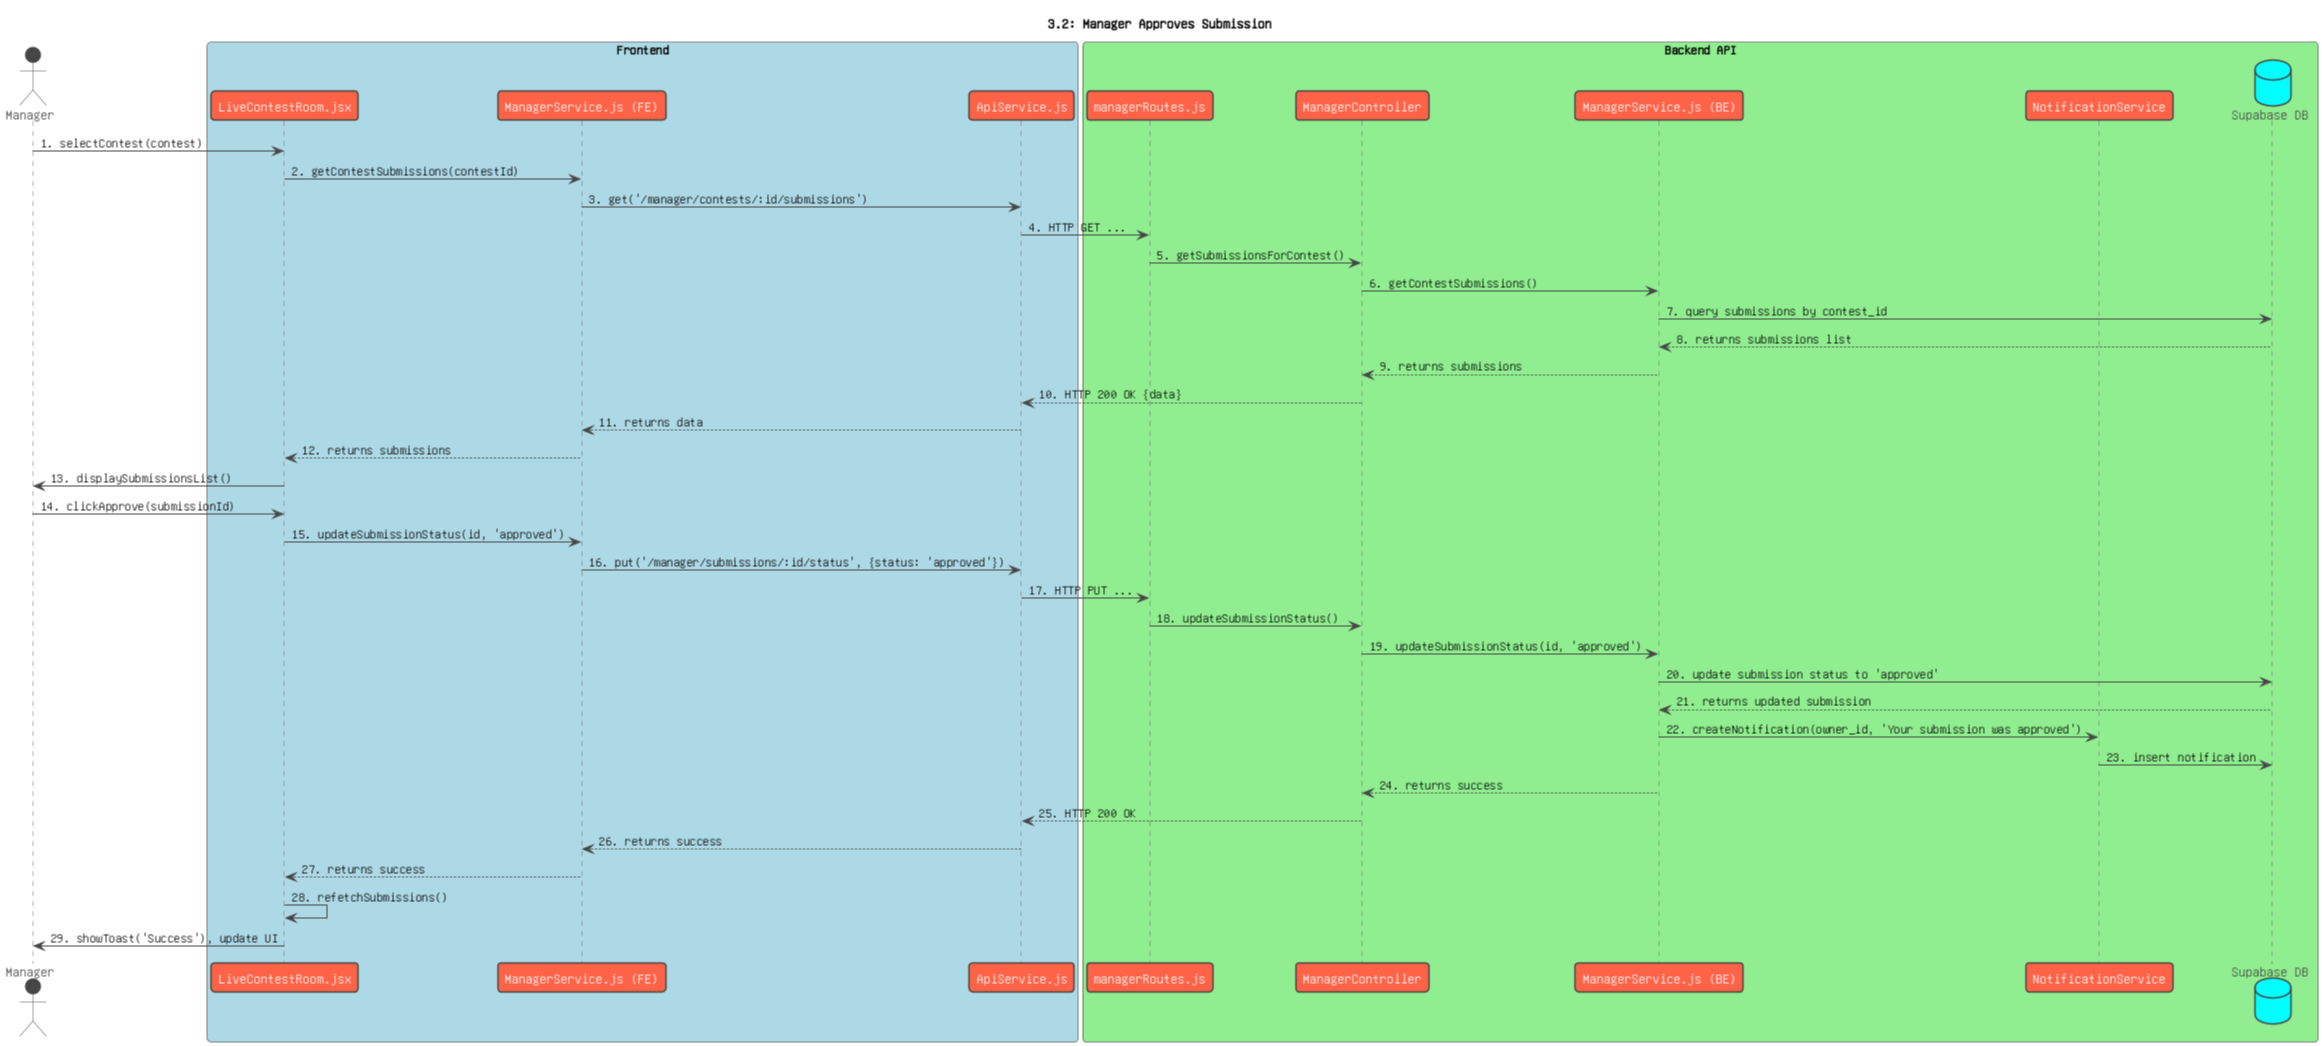
\includegraphics[width=0.8\linewidth]{S2.drawio}
	\caption{ขั้นตอนการส่งปลากัดเพื่อประเมิน (พร้อม AI)}
\end{figure}

\indent ไดอะแกรมนี้แสดงขั้นตอนที่ซับซ้อนขึ้น โดยแบ่งเป็น 2 ส่วน คือ การวิเคราะห์ด้วย AI (เกิดขึ้นเมื่ออัปโหลดรูป) และการส่งฟอร์มหลัก

\begin{sloppypar}
	\begin{enumerate}
		\item \textbf{ขั้นตอนการส่งปลากัดเพื่อประเมิน (พร้อม AI)}
		\begin{enumerate}
			\item การวิเคราะห์ด้วย AI (เกิดขึ้นอัตโนมัติเมื่อผู้ใช้อัปโหลดรูป)
			\begin{enumerate}
				\item User -> BettaEvaluationForm.jsx: ผู้ใช้เลือกไฟล์รูปภาพเพื่ออัปโหลด
				\item BettaEvaluationForm.jsx -> ModelService.js (FE): Component เรียกใช้ฟังก์ชัน analyzeBettaTypeAuto() เพื่อวิเคราะห์รูปภาพ
				\item ModelService.js (FE) -> ApiService.js: Service ของ Model เรียก ApiService เพื่อส่ง POST request ไปยัง Backend ที่ endpoint /model/analyze-single
				\item ApiService.js -> modelRoutes.js (BE): Request เดินทางถึง Backend และถูกส่งต่อไปยัง ModelController
				\item ModelController -> ModelApiService.js (BE): Controller เรียกใช้ ModelApiService ซึ่งเป็น Service ที่เชื่อมต่อกับ AI ภายนอก
				\item ModelApiService.js (BE) -> HuggingFace API: ส่งรูปภาพไปวิเคราะห์ที่ HuggingFace API 
				\item HuggingFace API -> ModelApiService.js (BE): ส่งผลลัพธ์ (ประเภทปลา/ความน่าจะเป็น) กลับมา
				\item ModelApiService.js (BE) -> ModelController: จัดรูปแบบผลลัพธ์แล้วส่งกลับ
				\item ModelController -> ApiService.js: ส่งผลลัพธ์กลับไปยัง Frontend (HTTP 200 OK)
				\item ApiService.js -> ModelService.js (FE): ส่งต่อผลลัพธ์
				\item ModelService.js (FE) -> BettaEvaluationForm.jsx: ส่งคำแนะนำกลับไปให้ Component
				\item BettaEvaluationForm.jsx -> User: แสดงผลการวิเคราะห์ของ AI บนหน้าจอ
			\end{enumerate} 
\newpage
			\item \textbf{การส่งฟอร์มหลัก} 
				\begin{enumerate}
					\item User -> BettaEvaluationForm.jsx: ผู้ใช้กรอกข้อมูลที่เหลือจนครบถ้วน และกดปุ่ม "ส่งประเมิน"
					\item BettaEvaluationForm.jsx -> UserService.js (FE): Component เรียกใช้ submitBettaForEvaluation()
					\item UserService.js (FE) -> ApiService.js: Service เรียก ApiService เพื่อส่ง POST request ไปยัง /submissions/evaluate พร้อมข้อมูลทั้งหมดจากฟอร์ม
					\item ApiService.js -> submissionRoutes.js (BE): Request เดินทางถึง Backend
					\item submissionRoutes.js (BE) -> SubmissionController: Route ส่งต่อให้ SubmissionController
					\item SubmissionController -> Supabase Storage: Controller อัปโหลดไฟล์รูปภาพและวิดีโอ ไปยัง Supabase Storage
					\item Supabase Storage --> SubmissionController: Supabase Storage คืนค่า URL ของไฟล์ที่อัปโหลดสำเร็จกลับมา
					\item SubmissionController -> SubmissionService.js (BE): Controller เรียกใช้ SubmissionService พร้อมข้อมูลทั้งหมด (รวมถึง URL ของไฟล์)
					\item SubmissionService.js (BE) -> Supabase DB: SubmissionService เรียกใช้ฟังก์ชัน create\_full\_submission (RPC) ในฐานข้อมูลเพื่อบันทึกข้อมูล Submission
					\item Supabase DB --> SubmissionService.js (BE): ฐานข้อมูลคืนค่า submission\_id ใหม่ที่ถูกสร้างขึ้น
					\item SubmissionController -> AutoAssignmentService: Controller เรียกใช้ AutoAssignmentService แบบ Fire-and-forget (ทำงานเบื้องหลัง) เพื่อมอบหมายงานให้ Expert โดยอัตโนมัติ 
					\item AutoAssignmentService -> Supabase DB: Service นี้จะค้นหา Expert ที่เหมาะสมและสร้าง assignment ใหม่ในฐานข้อมูล
					\item SubmissionController --> ApiService.js: Controller ส่ง HTTP Response 201 Created กลับไปยัง Frontend เพื่อยืนยันว่าการส่งผลงานสำเร็จ
					\item ApiService.js --> UserService.js (FE): ApiService ส่งต่อผลลัพธ์
					\item UserService.js (FE) --> BettaEvaluationForm.jsx: Service แจ้งผลสำเร็จกลับไปที่ Component
					\item BettaEvaluationForm.jsx -> User: Component แสดงข้อความ "สำเร็จ" และเปลี่ยนหน้าไปยังหน้าประวัติ (/history)
				\end{enumerate}
		\end{enumerate}
	\end{enumerate}
\end{sloppypar}

\newpage

\vspace{\baselineskip}

\begin{figure}[h]
	\centering
	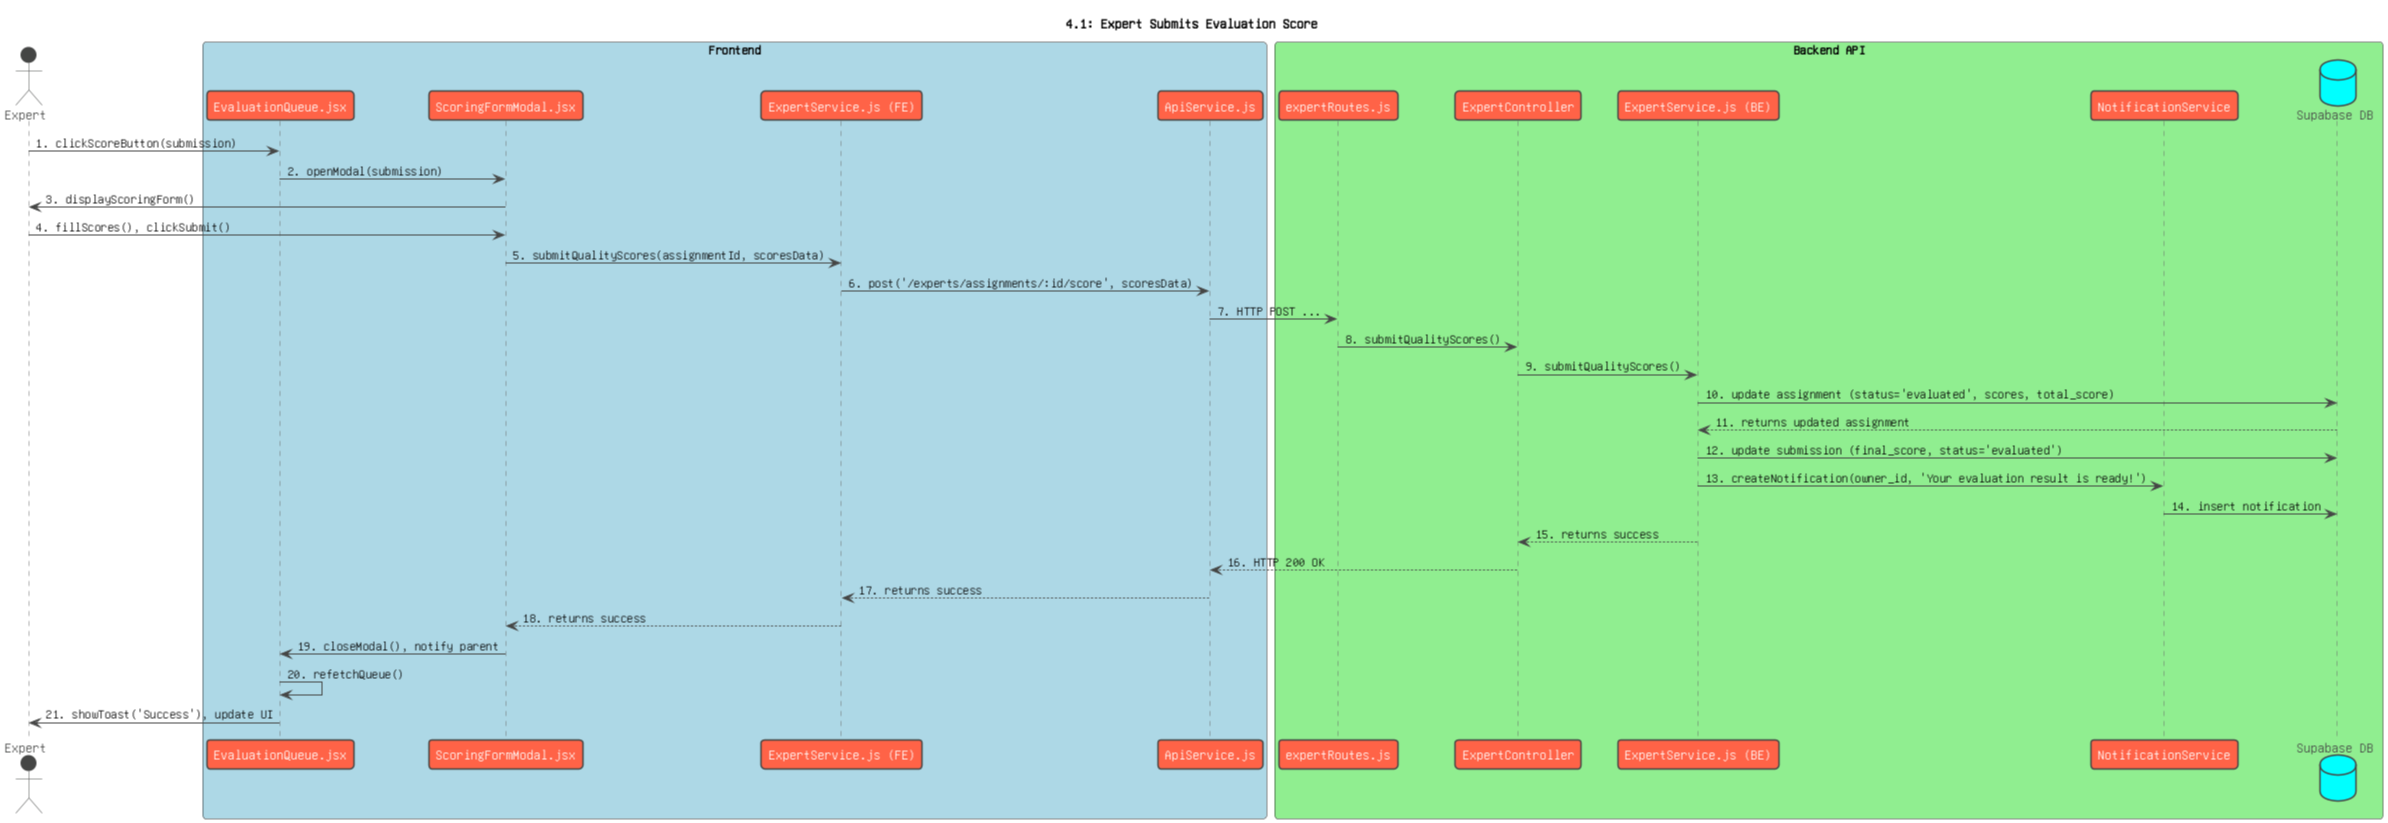
\includegraphics[width=0.8\linewidth]{S3.drawio}
	\caption{ขั้นตอนการอนุมัติผู้สมัครโดย Manager}
\end{figure}

\indent ไดอะแกรมนี้แสดงการทำงานในหน้า Live Contest Room เมื่อผู้จัดการทำการอนุมัติผู้ที่ส่งปลากัดเข้าร่วมการแข่งขัน

\begin{sloppypar}
	\begin{enumerate}
		\item Manager -> LiveContestRoom.jsx: ผู้จัดการเข้าสู่หน้า Live Room และเลือกการแข่งขันที่ต้องการจะดู
		\item LiveContestRoom.jsx -> ManagerService.js (FE): Component เรียกฟังก์ชัน getContestSubmissions() เพื่อขอดูรายชื่อผู้สมัครทั้งหมด
		\item ManagerService.js (FE) -> ApiService.js: Service ส่ง GET request ไปยัง Backend 
		\item ApiService.js -> managerRoutes.js (BE): Request เดินทางถึง Backend
		\item managerRoutes.js (BE) -> ManagerController: Route ส่งต่อให้ ManagerController
		\item ManagerController -> ManagerService.js (BE): Controller เรียก Service เพื่อดึงข้อมูล
		\item ManagerService.js (BE) -> Supabase DB: Service ค้นหาข้อมูล submissions ทั้งหมดที่เกี่ยวข้องกับการแข่งขันนี้จากฐานข้อมูล
		\item Supabase DB --> ManagerService.js (BE): ฐานข้อมูลส่งรายชื่อผู้สมัครกลับมา 
		\item ManagerService.js (BE) --> ManagerController: Service ส่งข้อมูลกลับให้ Controller
		\item ManagerController --> ApiService.js: Controller ส่ง HTTP Response 200 OK พร้อมรายชื่อผู้สมัครกลับมา
		\item ApiService.js --> ManagerService.js (FE): ApiService ส่งต่อข้อมูล
		\item ManagerService.js (FE) --> LiveContestRoom.jsx: Service ส่งข้อมูลกลับให้ Component
		\item LiveContestRoom.jsx -> Manager: Component แสดงรายชื่อผู้สมัครทั้งหมดบนหน้าจอ
		\item Manager -> LiveContestRoom.jsx: ผู้จัดการกดปุ่ม "อนุมัติ" บนรายการของผู้สมัครที่ต้องการ
		\item LiveContestRoom.jsx -> ManagerService.js (FE): Component เรียกฟังก์ชัน updateSubmissionStatus()
		\item ManagerService.js (FE) -> ApiService.js: Service ส่ง PUT request ไปยัง Backend เพื่ออัปเดตสถานะ
		\item ApiService.js -> managerRoutes.js (BE): Request เดินทางถึง Backend
		\item managerRoutes.js (BE) -> ManagerController: Route ส่งต่อให้ ManagerController
		\item ManagerController -> ManagerService.js (BE): Controller เรียก Service เพื่ออัปเดตสถานะ
		\item ManagerService.js (BE) -> Supabase DB: Service อัปเดตสถานะของ submission ในฐานข้อมูลเป็น 'approved'
		\item Supabase DB --> ManagerService.js (BE): ฐานข้อมูลยืนยันการอัปเดต
		\item ManagerService.js (BE) -> NotificationService: ManagerService เรียก NotificationService เพื่อสร้างการแจ้งเตือน
		\item NotificationService -> Supabase DB: Service บันทึกการแจ้งเตือนใหม่ ลงในฐานข้อมูลเพื่อส่งให้ผู้สมัคร
		\item ManagerService.js (BE) --> ManagerController: ManagerService แจ้งผลสำเร็จกลับ
		\item ManagerController --> ApiService.js: Controller ส่ง HTTP Response 200 OK
		\item ApiService.js --> ManagerService.js (FE): ApiService ส่งต่อผลลัพธ์
		\item ManagerService.js (FE) --> LiveContestRoom.jsx: Service แจ้งผลสำเร็จกลับไปที่ Component
		\item LiveContestRoom.jsx -> LiveContestRoom.jsx: Component เรียกข้อมูลผู้สมัครใหม่อีกครั้ง เพื่อให้หน้าจอเป็นข้อมูลล่าสุด
		\item LiveContestRoom.jsx -> Manager: Component แสดงข้อความ "สำเร็จ" และอัปเดต UI (เช่น ย้ายผู้สมัครจากแท็บ "รออนุมัติ" ไปยัง "อนุมัติแล้ว")
	\end{enumerate}
\end{sloppypar}
\vspace{\baselineskip}

\endgroup